\chapter{Comunicaciones}
\label{chap:robot}


En el presente capítulo comenzaremos con una introducción del funcionamiento y los fundamentos teóricos de cómo se gestionan las diferentes conexiones y eventos del framework para,
posteriormente, centrarnos en el ámbito específico de este proyecto con la finalidad de comprender mejor su funcionamiento.


\subsection{Fundamentos}
\label{sec:fundamentos}

En esta sección se describe cómo Sails trabaja con websocket y socket.io. Para ello se explicará con un ejemplo que facilite su comprensión.

Bien, pero ¿qué diablos son los eventos en tiempo real del modelo? Al igual que creamos manejadores de eventos para eventos DOM usando jquery, voy a mostrar un patrón para configurar los controladores de eventos para los cambios en los modelos que se emiten a cualquier socket que esté suscrito al evento.

REVISAR INTRODUCCION http://irlnathan.github.io/sailscasts/blog/2013/10/10/building-a-sails-application-ep21-integrating-socket-dot-io-and-sails-with-custom-controller-actions-using-real-time-model-events/



Centrémonos en el modelo usuario de RobotUI. Uno de sus atributos de este modelo es un booleano \emph{online}, el cual representa si un usuario se encuentra logueado en el sistema. Uno de los objetivos 
es saber cuando el usuario cambia el estado para poder proporcionar una actualización en tiempo real de la página de gestión de usuarios siempre y cuando un usuario inicie sesión o salga de la 
aplicación alternando entre las imágenes online: \icontext{.2}{.35}{imagenes/comunicaciones/online.png} y offline: \icontext{.2}{.35}{imagenes/comunicaciones/offline.png} sin necesidad de refrescar la página manualmente.\\

\begin{figure}[H]
  \begin{center}
    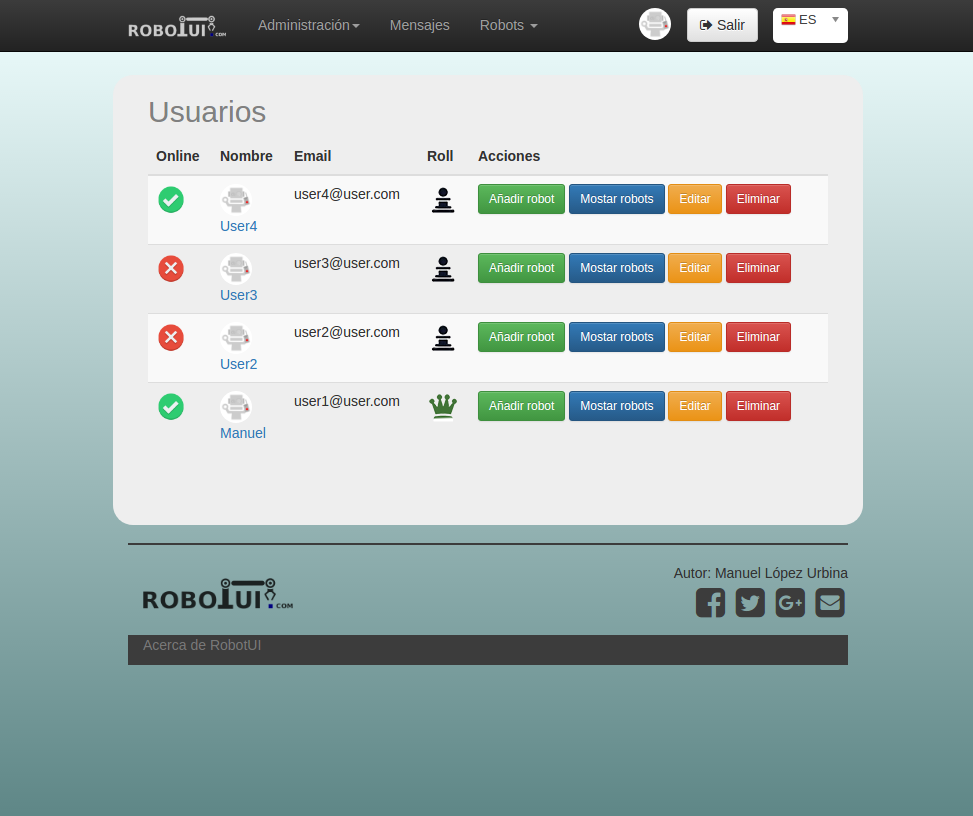
\includegraphics[scale=0.35]{imagenes/comunicaciones/index-usuarios.png}
  \end{center}
  \caption{Página de gestión de usuarios actualizable en tiempo real.}
  \label{view:userindex}
\end{figure}



\subsection{ Comunicaciones en RobotUI}
\label{sec:comunicaciones-robotui}


\begin{figure}[H]
  \begin{center}
    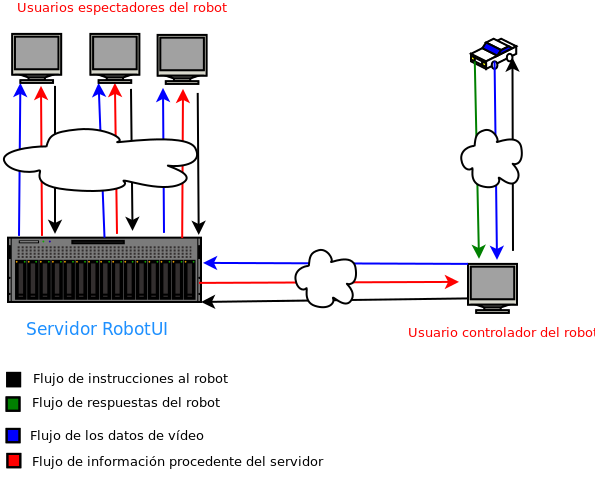
\includegraphics[scale=0.5]{diagramas/flujo-comunicaciones.png}
  \end{center}
  \caption{Esquema representativo del flujo de conexiones de RobotUI.}
  \label{diagram:conexiones}
\end{figure}
 

\subsubsection{ Conexión }
\label{sec:conexion}


Cuando se realiza una una conexión de un usuario al sistema, un nuevo cliente, realiza una petición al servidor, el cual captura la llamada y renderiza la vista correspondiente elaborando una respuesta.\\

Dicha respuesta se corresponde con el cógido Html y JavaScript que recibe el navegador. En el archivo \emph{views/layout.js} se encuentra el siguiente código JavaScript de gran importancia
para el funcionamiento de toda la aplicación por lo que resulta interesante su comprensión.\\

Primeramente al realizarse una nueva conexión de un cliente en el sistema el servidor debe conocer y registrar a dicho cliente con la finalidad de seguir su comportamiento, sus acciones y 
movimientos por toda la aplicación.\\

\begin{lstlisting}[language=JavaScript]
  //Funcion para tener en todo momento almacenado en la tabla session los sockets conectados junto con el usuario al que pertenece
  function savesocket() {
    io.socket.get("/session/saveSocketID");
  }  
\end{lstlisting}


Función que realiza el registro de un nuevo cliente en la base de datos:\\

\begin{lstlisting}[language=JavaScript]

  //Almacenamiento en la base de datos la sesion de cada usuario de la página:
  saveSocketID: function(req, res) {
    if (!req.isSocket) return res.badRequest();

    var socketId = sails.sockets.id(req);
    // => "BetX2G-2889Bg22xi-jy"

    if(req.session.User != undefined) {
      var sessionObj = {
        socket_id: socketId,
        user_id: req.session.User.id

      };

      //Comprobar si el usuario tiene sockets abiertos:
      Session.count({user_id: req.session.User.id}).exec(function countUserSessions(error, n_sessions) {
        console.log('There are ' + n_sessions + ' sessions of user ' + req.session.User.id);

        if (n_sessions == 0) {
          //Cambio de estado del usuario a online:
          User.update(req.session.User.id, {online: true}, function (err) {
            if (err) return res.badRequest();

            //Informar a otros clientes (sockets abiertos) que el usuario esta logueado:
            User.publishUpdate(req.session.User.id, {
              loggedIn: true,
              id: req.session.User.id
            });
          });
        }
      });

    }else {
      var sessionObj = {
        socket_id: socketId
      };
    }

    Session.create(sessionObj).exec( function (err, session) {
      if (err) return res.badRequest();

      console.log('\n..................................................');
      console.log('Conectando con Sails js.............................');
      console.log('Cliente conectado - id del socket: ' + socketId );
      console.log('....................................................');

      return;
    });
  },


\end{lstlisting}

Una vez finaliza el registro en el servidor del nuevo cliente se comprueba si existe definida la función \emph{subscribeAndListen} llamándose en caso afirmativo. Dicha función es específica para cada
funcionalidad que queramos inicializar o a qué eventos nos deseemos suscribir. Por ejemplo, suscibirnos a los eventos de conexión y desconexión de usuarios del panel de administración descrito en el apartado
\ref{sec:fundamentos} mediante la definición de la función \emph{subscribeAndListen} en la vista correspondiente.\\


Por otro lado, siempre se realiza la llamada a la función \emph{listenMessages} ya que independientemente de la vista en la que nos encontremos siempre nos mantendremos a la escucha de los mensajes 
recibidos a nuestra bandeja de entrada por parte de otros usuarios.\\

Finalmente mostramos el código JavaScript al completo localizado en el archivo \emph{views/layout.js}:\\


\begin{lstlisting}[language=JavaScript]

<script type="text/javascript">

  $.when(savesocket()).done(function(){
    if (typeof subscribeAndListen == 'function') {
      subscribeAndListen();
    }
    listenMessages();
  });

  //Funcion para tener en todo momento almacenado en la tabla session los sockets conectados junto con el usuario al que pertenece
  function savesocket() {
    io.socket.get("/session/saveSocketID");
  }

  //Evento a la espera de recibir mensajes y notificar al usuario:
  function listenMessages(){
    io.socket.on('user', function messageReceived(message) {
      switch (message.verb) {
        case 'messaged':
          var pathname = window.location.pathname;
          if(pathname == '/message/index'){
            location.reload();
          }else{
            new_msg_num_update('<%= i18n('messages') %>');
          }
          toastr.info('You have a new message! <a href="/message/show/' + message.data.msg.id + '"><%= i18n('open_here')%></a>' , 'Message');

          break;
        default:
          break;
      }
    });
  }

</script>
 
\end{lstlisting} 
 
\subsubsection { Desconexión }
\label{sec:deconexion}


En este apartado describiremos los puntos de mayor relevancia a la hora de la desconexión de alguna de las diferentes comunicaciones establecidas comenzando con la desconexión de un usuario.\\

Cuando un usuario realiza una desconexión, bien deslogueándose de la página o cerrando una de las ventanas abiertas, automáticamente se lanza una llamada a la 
función \emph{afterDisconnect} localizada en el fichero \emph{config/Socket.js} del servidor. Función que será ejecutada cada vez que un socket es desconectado del sistema.\\

Dicha función primeramente localiza qué sesión en la base de relacionada está relacionada con identificador del socket desconectado. Si este Socked estaba usando algún robot, éste se libera cambiando el estado
del robot a \emph{libre}. Y se informa a todos los sockets abiertos que el robot queda libreado y accesible al resto de usuarios.\\

\begin{lstlisting}[language=JavaScript]
  Robot.update({id: session.robot_id}, {busy: false}, function robotUpdated(err) {
    if (err) return next(err);

    //Informar a otros clientes (sockets abiertos) que el robot queda liberado
    Robot.publishUpdate(session.robot_id, {
      busy: false,
      id: session.robot_id
    });
  });
\end{lstlisting}


A continuación, se comprueba si el usuario no dispone de más sockets abiertos. Si fuera el caso de que no los disponga, entonces se procede a cambiar su estado a desconectado y se emite o se informa al resto de clientes (sockets abiertos)
que el usuario ya no se encuentra en el sistema. Llamada al método \emph{User.publishUpdate}: \\

\begin{lstlisting}[language=JavaScript]
   User.publishUpdate(session.user_id, {
    loggedIn: false,
    id: session.user_id
  });
\end{lstlisting}


Se comprueba si el usuario desconectado se encontraba en alguna \emph{room}. Pongamos como ejemplo que el usuario ha abandonado la visualización de un robot por lo queda
se debe informar a todos los sockets integrantes de esa \emph{room} que un usuario la ha abandonado con la función \emph{ sails.sockets.broadcast }. A continuación se muestra el fragmento de código:\\


\begin{lstlisting}[language=JavaScript]

//Emite a cada room que que se encuentre la sesión que un usuario la ha abandonado

session.rooms.forEach(function (room) {
  //sails.sockets.leave(session.socket_id, room.room_name, function(err) {
  //  if (err) {return res.serverError(err);}
  //});
  sails.sockets.broadcast(room.room_name, {type: 'exit', msg: {user_id: session.user_id}});
});

\end{lstlisting}



Finalmente se destruye la sesión:\\

\begin{lstlisting}[language=JavaScript]
    Session.destroy(session.id, function sessionDestroyed(err) {
      if (err) return cb();
      return cb();
    });
\end{lstlisting}


A continuación mostramos el código completo de la función \emph{afterDisconnect}:\\


\begin{lstlisting}[language=JavaScript]

  afterDisconnect: function(session, socket, cb) {
     console.log('Cliente desconectado - id del socket: ' + socket.id);

    //Session del socket cerrado,
    Session.findOne({socket_id: socket.id}).populate('rooms').exec(function (err, session) {
      if (err) return cb();
      if (!session) return cb();

      //Comprobar si el soscket estaba usando algun robot para liberarlo:
      if (session.robot_id) {
        console.log('Socked was using a robot');

        Robot.update({id: session.robot_id}, {busy: false}, function robotUpdated(err) {
          if (err) return next(err);

          //Informar a otros clientes (sockets abiertos) que el robot queda liberado
          Robot.publishUpdate(session.robot_id, {
            busy: false,
            id: session.robot_id
          });
        });
      }


      //Emite a cada room que que se encuentre la sesión que un usuario la ha abandonado ->  
      session.rooms.forEach(function (room) {
        //sails.sockets.leave(session.socket_id, room.room_name, function(err) {
        //  if (err) {return res.serverError(err);}
        //});
        sails.sockets.broadcast(room.room_name, {type: 'exit', msg: {user_id: session.user_id}});
      });


      //Comprobar si el usuario tiene más sockets abiertos:
      Session.count({user_id: session.user_id}).exec(function countUserSessions(error, n_sessions) {
        console.log('There are ' + n_sessions + ' users ' + session.user_id);

        //Cambiamos el usuario a offline si solo tenía una ventana o conexión abierta.
        if (n_sessions == 1) {
          User.update(session.user_id, {online: false}, function (err) {
            if (err) return cb(err);

            //Informar a otros clientes (sockets abiertos) que el usuario ya NO se encuentra logueado
            User.publishUpdate(session.user_id, {
              loggedIn: false,
              id: session.user_id
            });
          });
        }

        Session.destroy(session.id, function sessionDestroyed(err) {
          if (err) return cb();
          return cb();
        });
      });
    });
  }

\end{lstlisting}
 